\documentclass{standalone}
\usepackage{tikz}
\usetikzlibrary{patterns, positioning}
\usepackage[sfdefault]{ClearSans} %% option 'sfdefault' activates Clear Sans as the default text font
\usepackage[T1]{fontenc}

\begin{document}
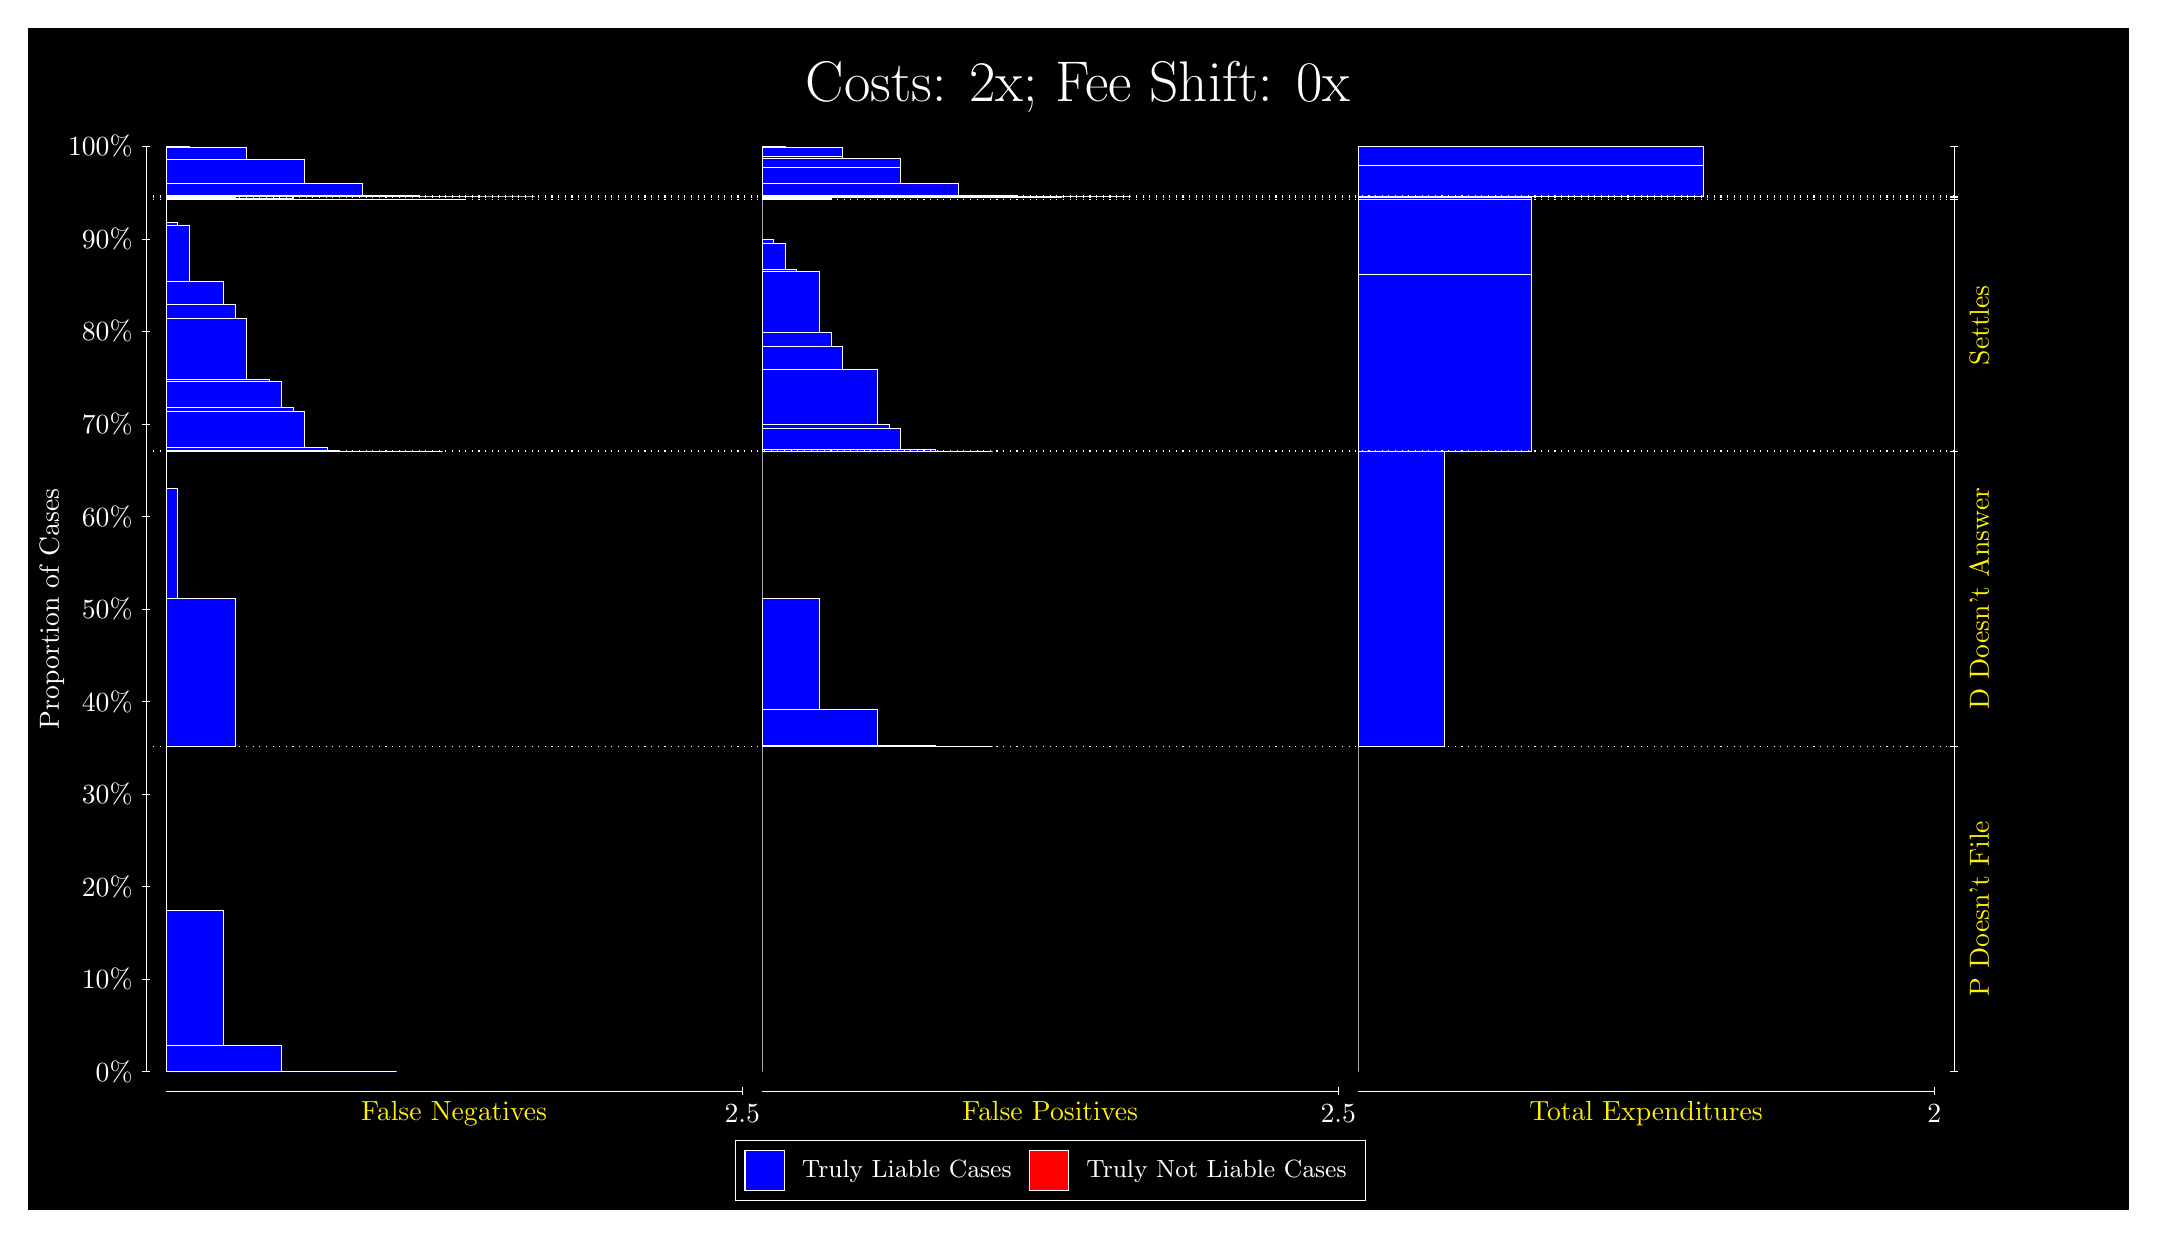
\begin{tikzpicture}
\draw[fill=black] (0,0) rectangle (26.667,15);
\draw[text=white] (0,13.5) rectangle (26.667,15) node[midway] {\huge Costs: 2x; Fee Shift: 0x};
\draw[white, very thin] (1.5,1.75) -- (1.5,13.5);
\node[rotate=90, text=white, anchor=center] at (0.3, 7.625) {Proportion of Cases};
\draw[white, very thin] (1.45,1.75) -- (1.55,1.75);
\node[text=white, anchor=east] at (1.45, 1.75) {0\%};
\draw[white, very thin] (1.45,2.925) -- (1.55,2.925);
\node[text=white, anchor=east] at (1.45, 2.925) {10\%};
\draw[white, very thin] (1.45,4.1) -- (1.55,4.1);
\node[text=white, anchor=east] at (1.45, 4.1) {20\%};
\draw[white, very thin] (1.45,5.275) -- (1.55,5.275);
\node[text=white, anchor=east] at (1.45, 5.275) {30\%};
\draw[white, very thin] (1.45,6.45) -- (1.55,6.45);
\node[text=white, anchor=east] at (1.45, 6.45) {40\%};
\draw[white, very thin] (1.45,7.625) -- (1.55,7.625);
\node[text=white, anchor=east] at (1.45, 7.625) {50\%};
\draw[white, very thin] (1.45,8.8) -- (1.55,8.8);
\node[text=white, anchor=east] at (1.45, 8.8) {60\%};
\draw[white, very thin] (1.45,9.975) -- (1.55,9.975);
\node[text=white, anchor=east] at (1.45, 9.975) {70\%};
\draw[white, very thin] (1.45,11.15) -- (1.55,11.15);
\node[text=white, anchor=east] at (1.45, 11.15) {80\%};
\draw[white, very thin] (1.45,12.325) -- (1.55,12.325);
\node[text=white, anchor=east] at (1.45, 12.325) {90\%};
\draw[white, very thin] (1.45,13.5) -- (1.55,13.5);
\node[text=white, anchor=east] at (1.45, 13.5) {100\%};

\draw[white, very thin] (24.457,1.75) -- (24.457,13.5);
\draw[white, very thin] (24.407,1.75) -- (24.507,1.75);
\node[anchor=west] at (24.407, 1.75) {};
\draw[white, very thin] (24.407,5.8812) -- (24.507,5.8812);
\node[anchor=west] at (24.407, 5.8812) {};
\draw[white, very thin] (24.407,9.631) -- (24.507,9.631);
\node[anchor=west] at (24.407, 9.631) {};
\draw[white, very thin] (24.407,12.826) -- (24.507,12.826);
\node[anchor=west] at (24.407, 12.826) {};
\draw[white, very thin] (24.407,12.851) -- (24.507,12.851);
\node[anchor=west] at (24.407, 12.851) {};
\draw[white, very thin] (24.407,12.869) -- (24.507,12.869);
\node[anchor=west] at (24.407, 12.869) {};
\draw[white, very thin] (24.407,13.5) -- (24.507,13.5);
\node[anchor=west] at (24.407, 13.5) {};

\draw[white, very thin, fill=blue] (1.75,1.75) rectangle (4.6775,1.75);
\draw[white, very thin, fill=blue] (1.75,1.75) rectangle (3.9457,1.7528);
\draw[white, very thin, fill=blue] (1.75,1.7528) rectangle (3.2138,2.0772);
\draw[white, very thin, fill=blue] (1.75,2.0772) rectangle (2.4819,3.8039);
\draw[white, very thin, fill=red] (1.75,3.8039) rectangle (1.75,3.8039);
\draw[white, very thin, fill=blue] (1.75,3.8039) rectangle (1.75,5.8812);
\draw[white, very thin, fill=blue] (1.75,5.8812) rectangle (2.6283,7.7551);
\draw[white, very thin, fill=blue] (1.75,7.7551) rectangle (1.8964,9.1572);
\draw[white, very thin, fill=red] (1.75,9.1572) rectangle (1.75,9.1572);
\draw[white, very thin, fill=blue] (1.75,9.1572) rectangle (1.75,9.631);
\draw[white, very thin, fill=blue] (1.75,9.631) rectangle (5.2631,9.631);
\draw[white, very thin, fill=blue] (1.75,9.631) rectangle (4.6775,9.631);
\draw[white, very thin, fill=blue] (1.75,9.631) rectangle (4.5312,9.6316);
\draw[white, very thin, fill=blue] (1.75,9.6316) rectangle (4.092,9.6328);
\draw[white, very thin, fill=blue] (1.75,9.6328) rectangle (3.9457,9.6459);
\draw[white, very thin, fill=blue] (1.75,9.6459) rectangle (3.7993,9.674);
\draw[white, very thin, fill=blue] (1.75,9.674) rectangle (3.5065,10.14);
\draw[white, very thin, fill=blue] (1.75,10.14) rectangle (3.3602,10.187);
\draw[white, very thin, fill=blue] (1.75,10.187) rectangle (3.2138,10.52);
\draw[white, very thin, fill=blue] (1.75,10.52) rectangle (3.0674,10.541);
\draw[white, very thin, fill=blue] (1.75,10.541) rectangle (2.7746,11.318);
\draw[white, very thin, fill=blue] (1.75,11.318) rectangle (2.6283,11.493);
\draw[white, very thin, fill=blue] (1.75,11.493) rectangle (2.4819,11.786);
\draw[white, very thin, fill=blue] (1.75,11.786) rectangle (2.3355,11.786);
\draw[white, very thin, fill=blue] (1.75,11.786) rectangle (2.0428,12.494);
\draw[white, very thin, fill=blue] (1.75,12.494) rectangle (1.8964,12.538);
\draw[white, very thin, fill=red] (1.75,12.538) rectangle (1.75,12.538);
\draw[white, very thin, fill=blue] (1.75,12.538) rectangle (1.75,12.826);
\draw[white, very thin, fill=blue] (1.75,12.826) rectangle (5.5558,12.826);
\draw[white, very thin, fill=blue] (1.75,12.826) rectangle (4.8239,12.826);
\draw[white, very thin, fill=blue] (1.75,12.826) rectangle (4.092,12.828);
\draw[white, very thin, fill=blue] (1.75,12.828) rectangle (3.3602,12.844);
\draw[white, very thin, fill=blue] (1.75,12.844) rectangle (2.6283,12.851);
\draw[white, very thin, fill=red] (1.75,12.851) rectangle (1.75,12.851);
\draw[white, very thin, fill=blue] (1.75,12.851) rectangle (2.6283,12.858);
\draw[white, very thin, fill=blue] (1.75,12.858) rectangle (1.8964,12.869);
\draw[white, very thin, fill=red] (1.75,12.869) rectangle (1.75,12.869);
\draw[white, very thin, fill=blue] (1.75,12.869) rectangle (1.75,12.869);
\draw[white, very thin, fill=blue] (1.75,12.869) rectangle (6.4341,12.869);
\draw[white, very thin, fill=blue] (1.75,12.869) rectangle (5.7022,12.869);
\draw[white, very thin, fill=blue] (1.75,12.869) rectangle (4.9703,12.878);
\draw[white, very thin, fill=blue] (1.75,12.878) rectangle (4.2384,13.025);
\draw[white, very thin, fill=blue] (1.75,13.025) rectangle (3.5065,13.341);
\draw[white, very thin, fill=blue] (1.75,13.341) rectangle (2.7746,13.488);
\draw[white, very thin, fill=blue] (1.75,13.488) rectangle (2.0428,13.5);
\draw[white, very thin, fill=red] (1.75,13.5) rectangle (1.75,13.5);
\draw[white, very thin, fill=blue] (1.75,13.5) rectangle (1.75,13.5);
\draw[white, very thin, fill=red] (9.3189,1.75) rectangle (9.3189,1.75);
\draw[white, very thin, fill=blue] (9.3189,1.75) rectangle (9.3189,5.8812);
\draw[white, very thin, fill=red] (9.3189,5.8812) rectangle (12.246,5.8812);
\draw[white, very thin, fill=blue] (9.3189,5.8812) rectangle (12.246,5.8812);
\draw[white, very thin, fill=blue] (9.3189,5.8812) rectangle (11.515,5.8929);
\draw[white, very thin, fill=blue] (9.3189,5.8929) rectangle (10.783,6.355);
\draw[white, very thin, fill=blue] (9.3189,6.355) rectangle (10.051,7.7571);
\draw[white, very thin, fill=blue] (9.3189,7.7571) rectangle (9.3189,9.631);
\draw[white, very thin, fill=red] (9.3189,9.631) rectangle (12.246,9.631);
\draw[white, very thin, fill=blue] (9.3189,9.631) rectangle (12.246,9.631);
\draw[white, very thin, fill=red] (9.3189,9.631) rectangle (11.661,9.631);
\draw[white, very thin, fill=blue] (9.3189,9.631) rectangle (11.661,9.6321);
\draw[white, very thin, fill=blue] (9.3189,9.6321) rectangle (11.515,9.6584);
\draw[white, very thin, fill=red] (9.3189,9.6584) rectangle (11.075,9.6584);
\draw[white, very thin, fill=blue] (9.3189,9.6584) rectangle (11.075,9.9196);
\draw[white, very thin, fill=blue] (9.3189,9.9196) rectangle (10.929,9.9637);
\draw[white, very thin, fill=blue] (9.3189,9.9637) rectangle (10.783,10.671);
\draw[white, very thin, fill=red] (9.3189,10.671) rectangle (10.49,10.671);
\draw[white, very thin, fill=blue] (9.3189,10.671) rectangle (10.49,10.671);
\draw[white, very thin, fill=blue] (9.3189,10.671) rectangle (10.344,10.964);
\draw[white, very thin, fill=blue] (9.3189,10.964) rectangle (10.197,11.14);
\draw[white, very thin, fill=blue] (9.3189,11.14) rectangle (10.051,11.916);
\draw[white, very thin, fill=blue] (9.3189,11.916) rectangle (9.758,11.937);
\draw[white, very thin, fill=blue] (9.3189,11.937) rectangle (9.6116,12.27);
\draw[white, very thin, fill=blue] (9.3189,12.27) rectangle (9.4652,12.317);
\draw[white, very thin, fill=blue] (9.3189,12.317) rectangle (9.3189,12.826);
\draw[white, very thin, fill=red] (9.3189,12.826) rectangle (10.197,12.826);
\draw[white, very thin, fill=blue] (9.3189,12.826) rectangle (10.197,12.834);
\draw[white, very thin, fill=blue] (9.3189,12.834) rectangle (9.4652,12.85);
\draw[white, very thin, fill=blue] (9.3189,12.85) rectangle (9.3189,12.851);
\draw[white, very thin, fill=red] (9.3189,12.851) rectangle (13.125,12.851);
\draw[white, very thin, fill=blue] (9.3189,12.851) rectangle (13.125,12.851);
\draw[white, very thin, fill=blue] (9.3189,12.851) rectangle (12.393,12.851);
\draw[white, very thin, fill=blue] (9.3189,12.851) rectangle (11.661,12.852);
\draw[white, very thin, fill=blue] (9.3189,12.852) rectangle (10.929,12.862);
\draw[white, very thin, fill=blue] (9.3189,12.862) rectangle (10.197,12.869);
\draw[white, very thin, fill=red] (9.3189,12.869) rectangle (14.003,12.869);
\draw[white, very thin, fill=blue] (9.3189,12.869) rectangle (14.003,12.869);
\draw[white, very thin, fill=red] (9.3189,12.869) rectangle (13.271,12.869);
\draw[white, very thin, fill=blue] (9.3189,12.869) rectangle (13.271,12.869);
\draw[white, very thin, fill=red] (9.3189,12.869) rectangle (12.539,12.869);
\draw[white, very thin, fill=blue] (9.3189,12.869) rectangle (12.539,12.881);
\draw[white, very thin, fill=blue] (9.3189,12.881) rectangle (11.807,13.027);
\draw[white, very thin, fill=red] (9.3189,13.027) rectangle (11.807,13.027);
\draw[white, very thin, fill=blue] (9.3189,13.027) rectangle (11.807,13.028);
\draw[white, very thin, fill=blue] (9.3189,13.028) rectangle (11.075,13.236);
\draw[white, very thin, fill=red] (9.3189,13.236) rectangle (11.075,13.236);
\draw[white, very thin, fill=blue] (9.3189,13.236) rectangle (11.075,13.344);
\draw[white, very thin, fill=blue] (9.3189,13.344) rectangle (10.344,13.368);
\draw[white, very thin, fill=blue] (9.3189,13.368) rectangle (10.344,13.491);
\draw[white, very thin, fill=blue] (9.3189,13.491) rectangle (9.6116,13.491);
\draw[white, very thin, fill=blue] (9.3189,13.491) rectangle (9.6116,13.5);
\draw[white, very thin, fill=blue] (9.3189,13.5) rectangle (9.3189,13.5);
\draw[white, very thin, fill=red] (16.888,1.75) rectangle (16.888,1.75);
\draw[white, very thin, fill=blue] (16.888,1.75) rectangle (16.888,5.8812);
\draw[white, very thin, fill=red] (16.888,5.8812) rectangle (17.986,5.8812);
\draw[white, very thin, fill=blue] (16.888,5.8812) rectangle (17.986,9.631);
\draw[white, very thin, fill=red] (16.888,9.631) rectangle (19.083,9.631);
\draw[white, very thin, fill=blue] (16.888,9.631) rectangle (19.083,11.875);
\draw[white, very thin, fill=red] (16.888,11.875) rectangle (19.083,11.875);
\draw[white, very thin, fill=blue] (16.888,11.875) rectangle (19.083,12.826);
\draw[white, very thin, fill=red] (16.888,12.826) rectangle (19.083,12.826);
\draw[white, very thin, fill=blue] (16.888,12.826) rectangle (19.083,12.851);
\draw[white, very thin, fill=red] (16.888,12.851) rectangle (19.083,12.851);
\draw[white, very thin, fill=blue] (16.888,12.851) rectangle (19.083,12.869);
\draw[white, very thin, fill=red] (16.888,12.869) rectangle (21.279,12.869);
\draw[white, very thin, fill=blue] (16.888,12.869) rectangle (21.279,13.259);
\draw[white, very thin, fill=red] (16.888,13.259) rectangle (21.279,13.259);
\draw[white, very thin, fill=blue] (16.888,13.259) rectangle (21.279,13.5);
\draw[white, dotted] (1.5,5.8812) -- (24.457,5.8812);
\draw[white, dotted] (1.5,9.631) -- (24.457,9.631);
\draw[white, dotted] (1.5,12.826) -- (24.457,12.826);
\draw[white, dotted] (1.5,12.851) -- (24.457,12.851);
\draw[white, dotted] (1.5,12.869) -- (24.457,12.869);
\draw[white, very thin] (1.75,1.5) -- (9.0689,1.5);
\node[text=yellow, anchor=north] at (5.4094, 1.5) {False Negatives};
\draw[white, very thin] (9.0689,1.45) -- (9.0689,1.55);
\node[text=white, anchor=north] at (9.0689, 1.45) {2.5};

\draw[white, very thin] (9.3189,1.5) -- (16.638,1.5);
\node[text=yellow, anchor=north] at (12.978, 1.5) {False Positives};
\draw[white, very thin] (16.638,1.45) -- (16.638,1.55);
\node[text=white, anchor=north] at (16.638, 1.45) {2.5};

\draw[white, very thin] (16.888,1.5) -- (24.207,1.5);
\node[text=yellow, anchor=north] at (20.547, 1.5) {Total Expenditures};
\draw[white, very thin] (24.207,1.45) -- (24.207,1.55);
\node[text=white, anchor=north] at (24.207, 1.45) {2};

\node[text=yellow, centered, rotate=90] at (24.777, 3.8156) {P Doesn't File};
\node[text=yellow, centered, rotate=90] at (24.777, 7.7561) {D Doesn't Answer};
\node[text=yellow, centered, rotate=90] at (24.777, 11.229) {Settles};




\draw (12.978300999999998,1.5) node[draw=none] (baseCoordinate) {};
\begin{scope}[align=center]
        \matrix[scale=0.5, draw=white, below=0.5cm of baseCoordinate, nodes={draw}, column sep=0.1cm]{
            \node[rectangle, draw, minimum width=0.5cm, minimum height=0.5cm, fill=blue] {}; &
            \node[draw=none, font=\small, text=white] (B) {Truly Liable Cases}; &
            \node[rectangle, draw, minimum width=0.5cm, minimum height=0.5cm, fill=red] {}; &
            \node[draw=none, font=\small, text=white] (B) {Truly Not Liable Cases}; \\
            };
\end{scope}

\end{tikzpicture}
\end{document}